\chapter{Cooperation, Competition, and Levels of Selection}

\begin{kaichang}
That honey jar in the kitchen represents one of the insect world's most remarkable engineering projects. A tablespoon of honey takes roughly a dozen or more workers' lifetime efforts: one worker produces only about one-twelfth of a teaspoon in its life. They leave the hive, visit millions of flowers, transport nectar home, fan away water with their wings, and seal honey into wax cells---yet most of the fruits of their labor never reach their own mouths.

Stranger still, workers are all female but almost never lay eggs. Faced with danger, they readily deploy their stings. Honeybee stings are barbed, and after penetrating skin, they tear away with part of the bee's internal organs; the worker dies within hours. \textbf{Giving up reproduction and dying for the group}: Chapter 76's logic suggests selection should favor individuals leaving as many offspring as possible. Why has such an other-serving trait persisted for tens of millions of years instead of disappearing?

Do not turn to the answer yet. Write down your guess. At the chapter's end, we will return to the honey jar and discover that the solution explains not only bees but every cell in your body, and even cancer.
\end{kaichang}

\textbf{Translator safety note:} Observe bees without handling them or provoking stings. A sting can cause a severe allergic reaction; breathing difficulty, throat or tongue swelling, or collapse requires immediate emergency help. See \href{https://www.nhs.uk/conditions/anaphylaxis/}{NHS anaphylaxis guidance}.

\section{Cooperation and Competition Are Everywhere}

Zoom out to see how widespread cooperation is:

\begin{itemize}[itemsep=2pt]
\item Ants ``herd'' aphids on plant stems. Aphids suck sap and excrete sugary honeydew for ants; ants drive away ladybirds and protect them. One partner supplies sugar, the other troops.
\item Gray-green lichen on rocks is not one organism but a partnership of fungi and algae or cyanobacteria. The photosynthetic partner makes sugar; the fungus supplies shelter, water, and minerals. Separated, both struggle to survive in the wild.
\item Soybeans, peas, and peanuts bear root nodules housing rhizobia. These bacteria turn atmospheric nitrogen into plant-usable nutrients, while plants share photosynthetic sugars.
\item Trillions of gut bacteria help you break down dietary fiber and synthesize certain vitamins; you supply warmth, moisture, and regular meals.
\end{itemize}

Competition occupies the same stage: thousands of bees seek the same flowers, weeds and crops compete for light, water, and nitrogen, and bacterial strains contest every foothold along your intestinal wall. Cooperation and competition are not opposing worlds but two outcomes of the same familiar rule. In Chapter 76's terms, \textbf{heritable variation plus differential reproductive success produces evolution}.

Yet earlier chapters treated individuals as the units selected: a long-necked individual feeds better, a dark individual hides better. Workers challenge this default assumption: if selection acts on individuals, their altruism seems inexplicable. Our real question is therefore: \textbf{at what level does natural selection occur}---genes, individuals, or groups?

\section{Kin Selection: Helping Relatives Helps Your Copies}

In 1964, British biologist Hamilton offered a disarmingly clean answer: \textbf{a gene does not care whose body it inhabits}.

Recall Chapter 69: sexual reproduction combines half the genes from each parent. You therefore share, on average, $1/2$ of your genes with siblings, $1/8$ with first cousins, and $1/2$ with parents or children. This fraction is the \emph{coefficient of relatedness}, $r$. Imagine an animal choosing between fleeing to preserve its own genes and sounding an alarm that attracts predators and likely kills it but saves nearby relatives. Its own set disappears, yet relatives retain many identical copies. From the perspective of the genes' average fate, an alarm may be a good bargain.

\begin{qiaoliang}
Hamilton expressed the bargain in an inequality, now called \emph{Hamilton's rule}:
\[
rB > C
\]
Here $C$ is the cost to the actor's reproduction, $B$ the benefit to the recipient's reproduction, and $r$ their relatedness. When the inequality holds, a gene for helping relatives tends to increase in frequency.

How many first cousins must a self-sacrifice save to break even? Set $C=1$, losing all future reproduction, with cousin relatedness $r=1/8$ and benefit $B=1$ per life saved. Then $\frac{1}{8} \times N > 1$ requires $N>8$. Hence Haldane's half-joking remark, made before Hamilton's work: ``I would jump into a river for two brothers or eight cousins.'' Siblings have $r=1/2$, so two suffice; cousins require eight. These numbers are extremely simplified---real $B$ and $C$ rarely equal one---but capture the point: \textbf{closer kinship, lower costs, and larger benefits make altruistic behavior easier for evolution to retain}. This is \emph{kin selection}.
\end{qiaoliang}

Bees add an elegant complication. Bees and ants are \emph{haplodiploid}: fertilized eggs become females, queens or workers, while unfertilized eggs become males. A female receives her father's complete gene set, since he has only one, and half her mother's. A worker therefore shares an average of $3/4$ of its genes with sisters, more than the $1/2$ it would share with a daughter. Helping its queen mother raise another sister can thus be more profitable genetically than producing a daughter. This was once the classic explanation for sterile bee castes.

A qualification is necessary: recent decades showed that many solitary bees and ants are also haplodiploid, while some highly social insects, such as termites, are not. Most scientists now consider the $3/4$ coincidence less important than Hamilton's broader logic: \textbf{helping relatives helps other copies of one's own genes}. Haplodiploidy merely tightens one screw in that mechanism. Revising explanations with evidence is the method these chapters have demonstrated since Chapter 76.

Kin selection extends beyond insects. Ground squirrels sound alarm calls on spotting predators, increasing their own danger while relatives escape. In many birds, including some jays, young individuals postpone breeding and remain near their parents' nests to feed younger siblings. Helping follows the same kinship arithmetic.

\section{Reciprocity and Symbiosis: Unrelated Partners}

If cooperation required kinship, ants and aphids, fungi and algae, and humans and gut bacteria would remain unexplained. Unrelated partners follow two other routes.

The first is \emph{reciprocity}: I help you now, you help me later. Vampire bats provide a classic example. They must obtain blood nightly and may starve after two or three unsuccessful nights. Successful bats often regurgitate blood to roost mates that failed to feed, even nonrelatives. Field observations show preferential sharing with previous donors. Reciprocity requires three conditions: partners \textbf{meet repeatedly}, rather than transact once; they can \textbf{recognize each other}, preventing cheats from taking without returning; and the helper's \textbf{cost is smaller than} the recipient's benefit. A mouthful of blood is worth far more to a starving bat than to an overfed one. Together, these conditions can stabilize account-keeping cooperation.

The second route goes further: \emph{symbiosis}, in which two species' metabolisms interlock, each supplying what the other lacks. Soybean root nodules provide an excellent example and this chapter's hands-on observation.

\begin{shiyan}
\textbf{Observe Legume Root Nodules} (a safe field observation)

\textbf{Materials}: a legume such as field-edge clover, wild vetch, alfalfa, or a potted bean seedling; a small trowel; clean water in a basin; a magnifying glass; disposable gloves; and white paper.

\textbf{Procedure}: 1. Dig up the entire plant with its roots, choosing a small plant and preserving fine roots as far as possible. 2. Gently rinse soil away in water and spread the roots on the paper. 3. Use the magnifier to find millet-grain-sized swellings attached to the roots: nodules. Compare a nonlegume root, such as a small grass dug up alongside. 4. Gently split a larger nodule with a fingernail and inspect its interior.

\textbf{What to observe}: how many nodules are present, and are they on the main root or side roots? Split nodules often look pale red because of \emph{leghemoglobin}, a protein resembling animal hemoglobin, jointly produced by plant and bacteria to regulate oxygen and protect nitrogen fixation.

\textbf{Safety reminder}: wear gloves and wash with soap afterward. Never eat unidentified plants. Return plants afterward or dispose of them appropriately.
\end{shiyan}

Nodules carry out an important step in the book's chemical chain. Atmospheric \chem{N_2} is extremely stable: a triple bond joins the nitrogen atoms, and breaking it costs considerable energy, as the bond-energy discussion around Chapter 30 explained. Rhizobial \emph{nitrogenase} can do it, but at a price: reducing one \chem{N_2} to two ammonia molecules, \chem{NH_3}, consumes at least 16 ATP. The plant's photosynthetic sugar supplies the raw material for ATP. Plants provide sugar, bacteria provide nitrogen-fixing chemistry, and neither partner can do without the other. Agricultural legumes enrich soil through this symbiosis: nitrogen-containing material left after harvest can reduce fertilizer requirements.

\section{Ultimate Partnership: Becoming Part of a Whole}

Symbiosis can go further still: one partner moves inside the other and never leaves. This is history, not science fiction. Mitochondria in every cell of your body, Chapter 58's power stations, and chloroplasts in every leaf, Chapter 54's photosynthetic workshops, descend from free-living bacteria.

\begin{zhengju}
In 1967, American biologist Lynn Margulis, then publishing as Sagan, submitted a paper with a startling claim: mitochondria and chloroplasts originated as bacteria swallowed by cells but retained instead of digested. The paper was \textbf{rejected about fifteen times} before publication and dismissed by mainstream researchers as fanciful for years afterward.

Margulis was not merely imagining. She had testable observations. Both organelles possess an extra membrane, a double envelope whose inner layer resembles a bacterium's membrane and outer layer a host-made engulfing pocket. Each carries a small circular DNA molecule resembling bacterial rather than nuclear linear chromosomes. Their ribosome sizes resemble bacterial ones, and some antibiotics inhibiting bacterial ribosomes also inhibit mitochondrial ribosomes. They multiply by processes resembling bacterial fission, and cells cannot make mitochondria from scratch: existing mitochondria produce new ones. A swallowed-bacterium origin unified these findings, while alternatives struggled.

Decisive evidence awaited mature DNA sequencing. Comparing mitochondrial DNA with bacterial sequences placed its closest relationship among $\alpha$-proteobacteria; chloroplast sequences pointed to cyanobacteria. Their ancestral addresses had been found. Endosymbiotic origin is now textbook consensus, while finer questions remain, such as how genes moved stepwise into the nucleus and whether other cellular structures have endosymbiotic origins. Science has not answered everything.
\end{zhengju}

Notice how complete the outcome was: during prolonged partnership, most former bacterial genes were lost or transferred to the host nucleus. Corresponding proteins are now made in the cytoplasm and imported into mitochondria. Free bacteria became ``organs'' indispensable to the host. Competition moved from between species to within a larger individual: two former partners merged into a new, higher-level whole. This suggests that \textbf{life's greatest innovations often arose not from improved parts but from independent replicating units joining into new wholes}.

\section{At What Level Does Selection Act?}

We can now answer the central question. Arrange life's replicating units by their nested relationships:

\begin{center}
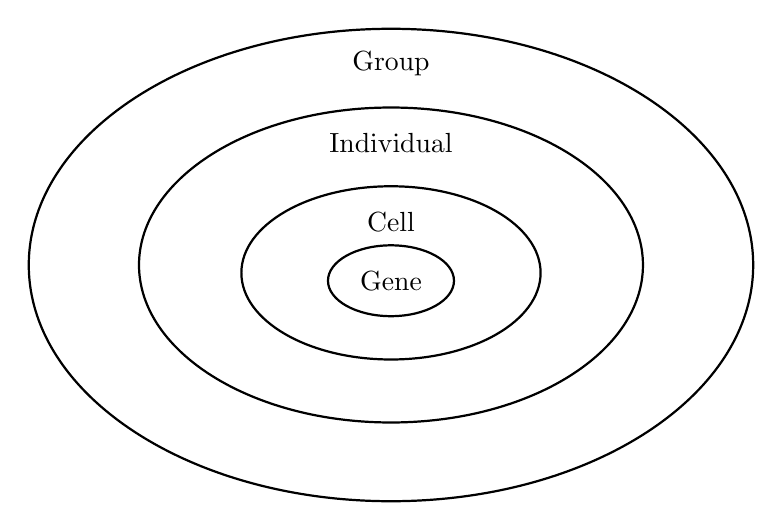
\begin{tikzpicture}[scale=1]
\draw[thick] (0,0) ellipse (4.6 and 3.0);
\draw[thick] (0,0) ellipse (3.2 and 2.0);
\draw[thick] (0,-0.1) ellipse (1.9 and 1.1);
\draw[thick] (0,-0.2) ellipse (0.8 and 0.45);
\node at (0,2.55) {Group};
\node at (0,1.55) {Individual};
\node at (0,0.55) {Cell};
\node at (0,-0.2) {Gene};
\end{tikzpicture}
\end{center}

(This is a representation: real groups, organisms, and cells are not tidy concentric circles, and their nesting is often more complex.)

\textbf{At the gene level}, selection favors sequences that increase their own copies. Last chapter's transposable elements succeed purely here: they do nothing for hosts but copy and paste themselves. Nearly half our genome records such freeloaders. Individual benefit alone cannot explain them; gene-level selection is required.

\textbf{At the individual level}, Darwin's familiar domain and earlier chapters' focus, long necks, protective coloration, and strong legs improve survival and reproduction.

\textbf{At the group level}, traits may harm individuals while helping groups, such as restrained reproduction that prevents resource exhaustion. In theory, if groups differ greatly and individuals frequently split and regroup, such traits may persist. This is \emph{group selection}. Its natural importance has been debated for decades without complete agreement. Most researchers consider it effective under restricted conditions, not an all-purpose explanation. This is a research frontier lacking a standard answer, not an omission from textbooks.

Crucially, these levels of selection \textbf{operate simultaneously and may point in opposite directions}. A gene-level winner, a transposon, may burden an individual; an individual-level loser, a stinging worker, may win at the gene level. Asking why a trait exists therefore raises at least three questions, beginning with the accounting level. This is the title's multilevel selection.

\begin{wuqu}
``The Selfish Gene shows organisms are innately selfish and every behavior is controlled by a particular selfish gene.'' This misreads the idea twice over. First, selfish genes are a metaphor: genes have no motives or wishes. The point is that inherited, replicable sequences form evolution's most stable accounting units. Second, that very logic predicts cooperation: kin selection, reciprocity, and symbiosis are routes selfish replicators take under particular conditions, as bees and vampire bats demonstrate. Third, real behavior is almost never one gene per action. Hundreds or thousands of genes, development, experience, and environment jointly shape it. Turning every behavior into one gene's strategy story is irresponsible simplification. A subtler related mistake assumes every trait must be adaptive. Chapter 77's drift and neutral evolution remind us that some are accidental or byproducts. Responsible evolutionary explanations need testable predictions; otherwise they are merely stories.
\end{wuqu}

\section{Cheats and Police Inside Multicellular Bodies}

Multilevel selection clarifies one of life's riskiest leaps: \textbf{from single cells to multicellular bodies}.

This happened independently many times, always confronting the same problem: each cell retains the ability to divide, so why not go it alone? A cell that divides recklessly and devotes all energy to copying itself wins internal competition in the short term. If every cell did so, however, the organism would collapse. In this chapter's terms, \textbf{cell-level selection favors cheating, while organism-level selection punishes it}. Multicellular life requires the higher level to restrain the lower.

Your body has a complete system of internal governance:

\begin{itemize}[itemsep=2pt]
\item \textbf{A single-cell bottleneck}: every generation starts again from one fertilized egg. As the previous chapter's embryonic development explained, tens of trillions of cells arise by clonal expansion from one cell and have almost identical genes. They are effectively one family with relatedness near one, removing the evolutionary incentive for internal competition: helping the body becomes their genes' only route forward. Moreover, new body-cell mutations cannot enter the next generation.
\item \textbf{Germline--soma division of labor}: only reproductive-lineage cells, future sperm or eggs, pass genes onward. However successful other cells become, their lines end. Like hive workers, body cells form a sterile caste serving the germline.
\item \textbf{Enforcement}: proteins such as p53 monitor DNA damage and trigger orderly cell suicide, apoptosis, when it cannot be repaired. Contact inhibition stops division when tissues become crowded, while immune surveillance removes abnormal cells.
\end{itemize}

Together, these reveal something striking: \textbf{your body is itself an evolved society}. Sterility, suicide, and policing nip selfish cellular winners in the bud. When this defense system occasionally fails, cancer results.

\section{Cancer: Evolution Within the Body}

Cancer is often called cellular rebellion, but we can be more precise: \textbf{cancer is evolution within a somatic-cell population}. Match the three requirements:

\begin{itemize}[itemsep=2pt]
\item \textbf{Variation}: copying errors during division, UV exposure, and tobacco chemicals, whose DNA damage Chapter 33 discussed, continually add somatic mutations.
\item \textbf{Selection}: most mutations are harmless or harmful, but a few hit key switches that let cells ignore stop signals, escape apoptosis, or evade immunity. Their bearers divide faster than neighbors and expand clonally. Tumors are not uniform masses but genetically differing clones \textbf{competing} for nutrients and space.
\item \textbf{Inheritance}: cells pass mutations to daughters, transmitting and amplifying advantageous clones' traits.
\end{itemize}

This explains a recurring clinical problem: chemotherapy or targeted drugs kill 99\% of tumor cells, but the few survivors carry resistance mutations and their clones return. It is \emph{the same} evolutionary logic as bacterial antibiotic resistance (Chapter 77), now staged inside the body. Researchers therefore investigate evolutionary approaches to treatment. Instead of trying to kill every tumor cell with one maximum dose, they adjust dosing schedules so sensitive cells restrain resistant ones and delay their expansion, an approach called adaptive therapy. These approaches remain in clinical trials with varying evidence levels. Individual treatment decisions belong to clinicians and patients using the evidence available at the time; a popular science book stops here.

\textbf{Translator safety note:} Do not skip doses, reduce doses, or interrupt cancer treatment to imitate this research. Adaptive therapy uses a defined clinical protocol with monitoring and eligibility criteria; it is not a general self-management strategy. Discuss options with the oncology team. See \href{https://www.cancer.gov/research/participate/clinical-trials-search/v?id=NCI-2024-06184}{NCI's adaptive-therapy trial description} and \href{https://www.cancer.gov/publications/patient-education/crs.pdf}{NCI clinical-trial guidance}.

To see why defenses must be so stringent, consider the scale:

\begin{qiaoliang}
Your genome contains about $3\times 10^{9}$ base pairs. Each body-cell division requires copying those three billion letters, with roughly $10^{-10}$ to $10^{-9}$ errors per copied base; proofreading and repair follow copying, as Chapter 66 explained. At this scale, \textbf{each division introduces about one new point mutation on average}. Bone marrow, gut epithelium, and skin divide extensively every day, totaling on the order of $10^{12}$ divisions body-wide. Today alone therefore produces roughly $10^{12}$ cells carrying new mutations. Over a year, almost every possible point mutation has appeared somewhere in you. The question becomes not why anyone gets cancer, but \textbf{why we do not all get it early}. The answer is layered defense: one cell must accumulate multiple particular mutations and escape apoptosis and immunity, each barrier reducing probability by several orders of magnitude. Cancer is an uncommon defensive failure, not the body's normal state.
\end{qiaoliang}

\section{Another Look at the Honey Jar}

Return to the puzzle: why do workers give up reproduction? A hive is a superorganism, with queen as germline and workers as body cells. The single-cell bottleneck, each colony beginning with one queen--male mating; kin selection, highly related sisters throughout the hive; and a new higher level, overwintering and defense by the whole colony, each correspond to our body's logic. Why have a barbed sting that kills its user? The relevant ledger is not the stinging bee's. After it dies, thousands of sisters with the same genes survive. Barbs are even good design: the embedded sting and venom sac keep pumping, injecting more venom and protecting the colony more thoroughly. Individual suicide earns a high gene-level score.

Honey is this superorganism's collective savings. No bee enjoys its entire labor's fruits or intends to dedicate itself to the group; bees do not have that intention. The order grows from a cold statistical rule: different fates of replicating units. This echoes Chapter 26: molecules do not want stability; low-energy states are statistically favored. Bees do not want sacrifice; colonies carrying these behavioral genes statistically leave more offspring. Anthropomorphism is a beginner's crutch; energy and statistics are the foundation.

\section{This Part Ends, and the Next Begins}

This part began with fossils and family trees and explored variation, selection, drift, speciation, and genomic remodeling before arriving at selection's levels. Evolution is far more than survival of the strong: cooperation and betrayal, levels and strategic interactions, controversy and uncertainty all feature. Every level connects to underlying chemistry: rhizobial ATP, nitrogenase breaking the nitrogen triple bond, and polymerases miscopying a base.

But notice a recurring kind of claim: comparing DNA reveals mitochondria's closest bacterial relatives. How can we read billions of bases? Once read, can they be edited? Could editing treat disease or improve crops, and what risks might arise? The next part, ``Reading and Writing Life, and Our Shared Future,'' begins here. Chapter 81 explains reading DNA, Chapter 82 rewriting genes, followed by gene therapy and agricultural and ecological choices. Anyone who understands this book will eventually help write it.

\section*{Try It Yourself}

\begin{sikaoti}
\item Draw gene flow among a hive's queen, workers, and drones. Why can sterile workers still help their genes reach the next generation?
\item An animal can sacrifice itself to save relatives. With full siblings ($r=1/2$), how many must survive to make this worthwhile under Hamilton's rule? What about nieces and nephews ($r=1/4$)? What simplifying assumptions does the calculation make?
\item Draw material flows in a root nodule, showing sugar and nitrogen-containing compounds passing between plant and rhizobia. Indicate the energy source driving each flow. (Hint: one requires ATP.)
\item Treat a growing tumor as an evolving population and draw its variation--selection--inheritance cycle. Show what happens to survivors after chemotherapy kills 99\% of cells. How does this resemble repeated use of one herbicide in a field?
\item ``Peacock tails make the species more beautiful'' and ``tears remove stress hormones'' exemplify what criticized explanatory error? Choose one and state a testable prediction that could turn it into a scientific hypothesis.
\item Use the nested-level diagram to explain why ``deer run fast so wolves do not eat the entire species'' is more questionable than ``the faster deer survived.'' Under what additional conditions could a group-benefit explanation hold?
\end{sikaoti}
